% EN49 c04 | 原书 原书 p.29–47（PDF 40–58） | 第 2 章 §2.1–2.3
% 骨架文件：标题行已设定，正文由译者填写。每页起首用 % ===== 原书 p.N ===== 注释标记。
\section{定义与约定}

\subsection{正合 Landau--Ginzburg 模型}

% ===== 原书 p.29 =====
首先说明如何把一个正合 Landau--Ginzburg 模型 $(X,W)$ 变成一个 Liouville 扇形，以便讨论它的 Fukaya--Seidel 范畴。

\begin{definition}\label{def:exact-lg}\label{def:2-1-1}
\textbf{正合 Landau--Ginzburg 模型}（exact Landau--Ginzburg model）$(X,W)$ 由以下数据构成：$X$ 是光滑仿射簇，带嵌入 $i\colon X\to\C^N$，该嵌入使 $X$ 成为 Stein 流形，其 Stein 函数 $\phi\colon X\to\R$ 取 $\phi(z)=|z|^2$ 在 $X$ 上的限制；此外还带全纯函数 $W\colon X\to\C$，它是 $\C^N$ 上某个多项式在 $X$ 上的限制。
\end{definition}

\transnote{易错预警：Stein 函数 $\phi$ 由标准欧氏范数 $|z|^2$ 限制得到，与 $W$ 无关；$|W|^2$ 只是实多项式，并不给出 Stein 结构。}

函数 $|W|^2$ 在 $\R^{2N}$ 上定义一个实多项式，而 $X\subseteq\R^{2N}$ 是实仿射代数簇。回忆：$|W|^2$ 在 $p\in\R$ 处的（实）Malgrange 条件，是指存在
% ===== 原书 p.30 =====
$R,\eps,\eta>0$，使得当 $|z|>R$ 且 $\bigl||W|^2(z)-p\bigr|\le\eps$ 时，有
\[
|z|\,\bigl|\nabla_X|W|^2\bigr|>\eta.
\]

\transnote{含糊点拨：Malgrange 条件是「在无穷远处 $\nabla_X|W|^2$ 不退化」的量化形式；三个常数 $R,\eps,\eta$ 彼此关联，不能独立选取。}

\begin{definition}\label{def:non-malgrange}\label{def:2-1-2}
若 $|W|^2$ 在 $p$ 处的 Malgrange 条件不成立，则称点 $p\in\R$ 为 $|W|^2\colon X\to\R$ 的\textbf{非 Malgrange 点}（non-Malgrange point）。类似地，若 $W$ 在 $p$ 处的（复）Malgrange 条件不成立，则称点 $p\in\C$ 为 $W\colon X\to\C$ 的非 Malgrange 点。
\end{definition}

实代数几何中有一个经典结论：使 $|W|^2\colon X\to\R$ 的 Malgrange 条件不成立的 $\R$ 中点只有有限多个（例如见 [Spo02, Remark 3]，再与代数簇 $X$ 取交）。类似地，$W$ 在 $\C$ 中的复非 Malgrange 点都是孤立的。

于是取 $R>0$ 充分大，使 $W$ 的全部临界点与非 Malgrange 点都落在 $|W|^2<R$ 之内。再把 $X$ 上的 Stein 结构 $\phi$ 形变为
\[
\psi_t(z)=\phi(z)+D\left(\frac{t+\phi(z)|W|^{2m}}{1+t\phi(z)|W|^{2m}}\right),
\]
其中 $t\in[0,1]$，$D>0$ 是正常数，$m$ 是正整数。则

\begin{lemma}\label{lem:psi-outward}\label{lem:2-1-3}
当 $R,D,m>0$ 充分大时，$\psi=\psi_0$ 的 Liouville 向量场沿 $|W|^2=R$ 指向外侧。
\end{lemma}

\begin{proof}
需要验证内积
\[
\langle\nabla_X|W|^2,\nabla_X\psi\rangle
=(1+D|W|^{2m})\langle\nabla_X|W|^2,\nabla_X\phi\rangle
+mD|W|^{2m-2}\phi\bigl|\nabla_X|W|^2\bigr|^2
\]
在 $|W|^2=R$ 上处处严格为正。
% ===== 原书 p.31 =====
由 Cauchy--Schwarz 不等式，
\[
(1+D|W|^{2m})\bigl|\langle\nabla_X|W|^2,\nabla_X\phi\rangle\bigr|
\le 2(1+D|W|^{2m})\bigl|\nabla_X|W|^2\bigr||\phi|^{1/2},
\]
因此只要
\[
2(1+D|W|^{2m})<mD|W|^{2m-2}|\phi|^{1/2}\bigl|\nabla_X|W|^2\bigr|
\]
就有 $\langle\nabla_X|W|^2,\nabla_X\psi\rangle>0$。利用
\[
|\nabla_X\phi|\le\bigl|\nabla|z|^2\bigr|=2|z|
\]
可把该不等式改写为
\begin{equation}\label{eq:2-1}
2\left(\frac{1}{D|W|^{2m-2}}+|W|^2\right)
<m|\phi|^{1/2}\bigl|\nabla_X|W|^2\bigr|.
\end{equation}

\transnote{易错预警：由 $|\nabla_X\phi|\le 2|z|$ 推出 (2.1)，这一步只用 $\C^N$ 的标准度量；换用别的 Kähler 度量，其中的常数要跟着变。}
当 Malgrange 条件在 $R$ 处成立时，存在常数 $\eta>0$，使 $|z|\bigl|\nabla_X|W|^2\bigr|>\eta$ 在 $|W|^2=R$ 上成立；若 $R$ 充分大，使 $W$ 在 $|W|^2=R$ 上没有临界点，则该处 $\bigl|\nabla_X|W|^2\bigr|>0$，于是存在常数 $C>0$（依赖于 $R$），使
\[
|W|^2<C|z|\bigl|\nabla_X|W|^2\bigr|.
\]
% ===== 原书 p.32 =====
因此当 $D,m>0$ 充分大时，不等式 \eqref{eq:2-1} 成立。
\end{proof}

类似地，我们还需要知道 $W$ 的平行移动在某个圆盘之外有定义：

\begin{lemma}\label{lem:parallel-transport}\label{lem:2-1-4}
对某个充分大的 $R>0$，辛平行移动在 $|W|^2=R$ 上方的 $W$ 的光滑纤维之间给出正合辛同胚。
\end{lemma}

\begin{proof}
我们沿用 [FSS08, §2] 的论证。由简单计算（参看 [Sei08b, p.213]）可知，只要辛平行移动有定义，它给出的就是正合辛同胚。平行移动向量场总是
\[
\frac{\nabla_X\operatorname{Re}(W)}{\bigl|\nabla_X\operatorname{Re}(W)\bigr|^2}
\]
的单位复数倍，因为 $\nabla_X\operatorname{Im}(W)=J\nabla_X\operatorname{Re}(W)$。由于 $\phi\colon X\to\R$ 是逆紧（proper）的穷竭函数，只需证明平行移动向量场的流线 $\gamma(t)$ 在 $\phi$ 下的像不会在有限时间内逃向无穷。于是考虑导数
\[
\left|\frac{\nabla_X\operatorname{Re}(W)}{\bigl|\nabla_X\operatorname{Re}(W)\bigr|^2}\phi\right|
=\frac{\bigl|\langle\nabla_X\operatorname{Re}(W),\nabla_X\phi\rangle\bigr|}
{\bigl|\nabla_X\operatorname{Re}(W)\bigr|^2}
\le\frac{|\nabla_X\phi|}{\bigl|\nabla_X\operatorname{Re}(W)\bigr|}.
\]
复多项式 $W\colon X\to\C$ 的 Malgrange 条件在 $\C$ 中只有有限多个点处不成立，故存在常数 $C>0$ 与 $R>0$，使
\[
|W|<C|\phi|^{1/2}|\de_XW|
\]
% ===== 原书 p.33 =====
对 $|W|=R$ 成立，其中 $|\de_XW|=\bigl|\nabla_X\operatorname{Re}(W)\bigr|$。另注意在 $\C^N$ 上有
\[
|\nabla\phi|=\bigl|\nabla|z|^2\bigr|=2|\phi|^{1/2},
\]
从而 $|\nabla_X\phi|\le2|\phi|^{1/2}$。因此在 $|W|=R$ 上，对某个常数 $C$ 有
\[
\phi'(t)\le C\frac{\phi(t)}{|W(t)|},
\]
其中 $\phi(t)=\phi(\gamma(t))$。若 $\gamma(t)$ 避开 $W$ 的零纤维，则存在常数 $\beta>0$，使 $1/|W(t)|<\beta$。于是由 Gr{\"o}nwall 不等式，
\[
\phi(t)\le\phi(0)e^{C\beta t},
\]
证毕。
\end{proof}

\transnote{背景直觉：Grönwall 不等式把 $\phi$ 沿流线的增长压到指数级；指数增长在有限时间内有界，因此流线逃不到无穷远。}

我们常常希望换用另一个 Stein 函数来计算深谷范畴。下面记录一条此后反复使用的标准引理；它在文献中只以隐含的形式出现。

\begin{definition}\label{def:simple-liouville}\label{def:2-1-5}
设 $X$ 是带 Liouville 形式 $\lambda$ 的 Liouville 流形。若 Liouville 形式的光滑族 $\lambda_t$（$t\in[0,1]$）满足 $\lambda_0=\lambda$，且各 Liouville 结构 $\lambda_t$ 的骨架之并始终含于某个紧集之内，则称该族为\textbf{简单 Liouville 同伦}（simple Liouville homotopy）。
\end{definition}

\transnote{含糊点拨：条件只要求「骨架之并」落在某个紧集之内，并不要求骨架本身逐点不动，所以允许骨架随 $t$ 移动。}

% ===== 原书 p.34 =====
例如，临界点始终留在紧集之内的一族 Weinstein 函数就满足这一条件。

\begin{lemma}\label{lem:simple-homotopy}\label{lem:2-1-6}
给定 Liouville 流形 $X$ 与简单 Liouville 同伦 $\lambda_t$，所有 Liouville 流形 $(X,\lambda_t)$ 彼此正合辛同胚，且 wrapped Fukaya 范畴 $\cW(X,\lambda_t)$ 彼此拟等价。
\end{lemma}

\begin{proof}
由 [CE12, Proposition 11.8]，对每个简单 Liouville 同伦，存在一族正合辛同胚 $\phi_t\colon X\to X$，满足 $\phi_t^*\lambda_t=\lambda-\de f$（$f$ 紧支），且 $\phi_0$ 为恒同。这给出 Liouville 扇形的一个平凡包含；故由 [GPS19, Lemma 2.6]，该形变给出 $\cW(X,\lambda_0)$ 与 $\cW(X,\lambda_1)$ 之间的拟等价。
\end{proof}

因此，只要只在拟等价意义下考虑深谷范畴（依据 [Sei08b, Corollary 1.14]），我们在证明中就可以自由使用形变后的 Liouville 结构。带停点的情形也有引理 \ref{lem:simple-homotopy} 的类似版本。这一自由度有一个特别好用的应用：

\begin{proposition}\label{prop:convex-boundary}\label{prop:2-1-7}
存在从 Stein 流形 $(X,\phi)$ 到 Stein 流形 $(X,\psi)$ 的简单 Liouville 形变，使得当 $R_1,R_2>0$ 充分大时，子集 $\{|W|^2\le R_1\}\cap\{\psi\le R_2\}$ 的边界为凸。此外，所有纤维 $W^{-1}(z)\cap\{\psi\le R_2\}$ 都经由沿 $|W|^2(z)=R_1$ 的辛平行移动而彼此正合辛同胚；把角磨圆、得到 Liouville 域
% ===== 原书 p.35 =====
$X_0$ 之后，它们仍彼此正合辛同胚。
\end{proposition}

把磨圆参数取得充分小，则 Liouville 域 $X_0$ 的接触边界包含 Liouville 超曲面 $F=W^{-1}(R_1)\cap\{\psi\le R_2-\eps\}$，且 $F$ 的边界为凸；还可取 $\eps>0$ 充分小，使 $F$ 的完备化与 $W^{-1}(R_1)$ 正合辛同胚。数对 $(X_0,F)$ 给出一个缝合 Liouville 域（sutured Liouville domain），它与充分大的 $R_1,R_2$ 无关。由 [GPS20a, Lemma 2.32]，缝合 Liouville 域对应一个（同伦意义下）唯一的 Liouville 扇形；我们把它记作 $(X,W)$。

\begin{definition}\label{def:liouville-sector}\label{def:2-1-8}
Landau--Ginzburg 模型 $(X,W)$ 所对应的 Liouville 扇形 $(X,W)$，是指（磨圆后的）缝合 Liouville 域
\[
\bigl(\{|W|^2\le R_1\}\cap\{\psi\le R_2\},\ W^{-1}(R_1)\cap\{\psi\le R_2-\eps\}\bigr)
\]
在 $R_1,R_2>0$ 充分大、$\eps>0$ 充分小时所对应的 Liouville 扇形的（等价类）。
\end{definition}

\begin{definition}\label{def:fs-category}\label{def:2-1-9}
$(X,W)$ 的\textbf{Fukaya--Seidel 范畴}，记作 $\cW(X,W)$，是指上述 Liouville 扇形 $(X,W)$ 依 [GPS20a] 意义的部分缠绕深谷范畴。
\end{definition}

这里要说明：把缝合 Liouville 域变成 Liouville 扇形有两种构造。其一是 [GPS20a, Definition 2.14] 所述的“完备化”。另一种是对 $F=W^{-1}(R_1)\cap\{\psi\le R_2-\eps\}$ 应用 [Syl19b, Prop 2.6]；在可能增大 $R_1,R_2$ 之后，由此得到 $F$ 的一个标准 Liouville 邻域 $U$，其形如
\[
\bigl(\hat F\times\{z\in\C:\operatorname{Re}(z)>-\rho\},\ \lambda_X|_F+\lambda_{\C}^{\mathrm{std}}\bigr),
\]
并真嵌入于完备化 $\hat X_0$ 之内，其中 $\rho>0$。此时超曲面 $\{\operatorname{Re}(z)=0\}$ 平行于无穷远处的 Liouville 向量场，并以 $I=\operatorname{Im}(z)$ 为定义函数（见 [GPS20a, Definition
% ===== 原书 p.36 =====
2.4]）。这就把 $\{\operatorname{Re}(z)\le0\}$ 变成了一个 Liouville 扇形。由 [GPS20a, Lemma 2.32]，存在（同伦意义下）唯一的 Liouville 扇形同伦，从 $\{\operatorname{Re}(z)\le0\}\subseteq\hat X_0$ 过渡到 $(X_0,F)$ 的凸完备化；细察该论证可见，这个同伦可取成简单 Liouville 同伦。

取光滑弧 $\gamma\colon[0,1]\to\C$，$\gamma(t)=R_1e^{i\theta(t)}$，其中 $\theta(t)=\delta+t(2\pi-\delta)$，$\delta>0$ 充分小。沿从 $1$ 到 $z$ 的射线（若这些射线恰好穿过 $W$ 的非 Malgrange 点，就取射线的小扰动）作平行移动，可把每个纤维 $F_z=W^{-1}(z)$ 与参考纤维 $F=W^{-1}(1)$ 等同起来。在这一等同之下，\textbf{逆时针整体单值性} $\mu\colon F\to F$ 定义为 $\Phi_\gamma\colon F_{R_1e^{i\delta}}\to F_{R_1}$ 所给出的平行移动辛同胚，其中 $W$ 的 $\delta>0$ 充分小。

\begin{remarkx}\label{rem:5}
本论文两部分所用的约定彼此相反：在第一部分，我们改取 $\mu$ 为\emph{顺时针}整体单值性，并把停点 $F$ 放在负实轴上的 $-R_1$ 处。这样选择的理由将在 §2.3 中说明。
\end{remarkx}

对于光滑环簇 Fano 簇的镜像 $((\C^*)^n,f)$，已知在 §1 的假设下，取 $T>0$ 充分小，可使 $f$ 的全部临界值落在 $1$ 的任意小邻域内（例如见 [Aur18, Lemma 5.2]）。注意 [Aur18] 假设了更强的条件 (2)：极大胞腔是幺模单形；而 [Aur18, Lemma 5.2] 的证明只用到较弱的那条假设，即它们是单形（见注 2）。于是可把 [Jef22] 中的上述论证用于 $W=1-f$，得知 $\{|f-1|\le R_1\}\cap\{\psi\le R_2\}$ 的边界为凸。总结如下：

% ===== 原书 p.37 =====
\begin{definition}\label{def:toric-lg-sector}\label{def:2-1-10}
Liouville 扇形 $((\C^*)^n,f)$ 的定义如下：在带标准 Stein 结构 $\phi$ 的 $(\C^*)^n$ 上，对函数 $1-f$ 应用定义 \ref{def:liouville-sector}，其中 $R_1>1$。所取的超曲面 $F$ 是一个 Liouville 域，其完备化与参考纤维 $H=f^{-1}(0)$ 同痕。
\end{definition}

\subsection{局部 Fukaya--Seidel 范畴}

在另一些场合，我们只关心 Landau--Ginzburg 模型在 $W$ 的单个奇点附近的局部辛行为。不妨设该奇点在 $0\in\C^N$，且 $W(0)=0$。此时我们希望只把 Liouville 扇形与这一个临界值联系起来。

仍如上面那样，由于使 $|W|^2$ 的 Malgrange 条件失效的 $W$ 值都是孤立的，可取 $\delta>0$ 严格小于 $\R_{>0}$ 中所有使 $|W|^2$ 的 Malgrange 条件失效的点。于是存在常数 $C$，使对一切 $0<|W|^2<\delta$ 有
\[
|W|^2<C|z|\bigl|\nabla_X|W|^2\bigr|.
\]
再把 $X$ 上的 Stein 结构 $\phi$ 形变为
\[
\psi_t(z)=\phi(z)+D\left(\frac{t+\phi(z)|W|^{2m}}{1+t\phi(z)|W|^{2m}}\right),
\]
其中 $t\in[0,1]$，$D>0$ 是正常数，$m$ 是正整数。则

\begin{lemma}\label{lem:local-psi-outward}\label{lem:2-2-1}
当 $D,m>0$ 充分大、$\delta>0$ 充分小时，$\psi=\psi_0$ 的 Liouville 向量场沿 $|W|^2=\delta$ 指向外侧。
\end{lemma}

% ===== 原书 p.38 =====
\begin{proof}
考察内积
\[
\langle\nabla_X|W|^2,\nabla_X\psi\rangle
=(1+D|W|^{2m})\langle\nabla_X|W|^2,\nabla_X\phi\rangle
+mD|W|^{2m-2}\phi\bigl|\nabla_X|W|^2\bigr|^2.
\]
由 Cauchy--Schwarz 不等式，
\[
(1+D|W|^{2m})\bigl|\langle\nabla_X|W|^2,\nabla_X\phi\rangle\bigr|
\le 2(1+D|W|^{2m})\bigl|\nabla_X|W|^2\bigr||\phi|^{1/2},
\]
因此只要
\[
2(1+D|W|^{2m})<mD|W|^{2m-2}|\phi|^{1/2}\bigl|\nabla_X|W|^2\bigr|
\]
就有 $\langle\nabla_X|W|^2,\nabla_X\psi\rangle>0$，这里用到
\[
|\nabla_X\phi|\le\bigl|\nabla|z|^2\bigr|=2|z|.
\]
把该不等式改写，得到
\[
2\left(\frac{1}{D|W|^{2m-2}}+|W|^2\right)
<m|\phi|^{1/2}\bigl|\nabla_X|W|^2\bigr|.
\]
若取 $D>1/\delta^m$，则
\[
\frac{1}{D|W|^{2m-2}}<\delta,
\]
% ===== 原书 p.39 =====
于是按我们的构造，
\[
4\delta<m|z|\bigl|\nabla_X|W|^2\bigr|
\]
成立。
\end{proof}

类似地，平行移动在局部也成立：

\begin{lemma}\label{lem:local-parallel-transport}\label{lem:2-2-2}
当 $\eps>0$ 充分小时，辛平行移动在 $0<|W|<\eps$ 上方 $W$ 的光滑纤维之间给出正合辛同胚。
\end{lemma}

\begin{proof}
我们沿用 [FSS08, §2] 的论证。由简单计算（参看 [Sei08b, p.213]）可知，只要辛平行移动有定义，它给出的就是正合辛同胚。平行移动向量场总是
\[
\frac{\nabla_X\operatorname{Re}(W)}{\bigl|\nabla_X\operatorname{Re}(W)\bigr|^2}
\]
的单位复数倍，因为 $\nabla_X\operatorname{Im}(W)=J\nabla_X\operatorname{Re}(W)$。由于 $\phi\colon X\to\R$ 是逆紧的穷竭函数，只需证明平行移动向量场的流线 $\gamma(t)$ 在 $\phi$ 下的像不会在有限时间内逃向无穷。于是考虑导数
\[
\left|\frac{\nabla_X\operatorname{Re}(W)}{\bigl|\nabla_X\operatorname{Re}(W)\bigr|^2}\phi\right|
=\frac{\bigl|\langle\nabla_X\operatorname{Re}(W),\nabla_X\phi\rangle\bigr|}
{\bigl|\nabla_X\operatorname{Re}(W)\bigr|^2}
\le\frac{|\nabla_X\phi|}{\bigl|\nabla_X\operatorname{Re}(W)\bigr|}.
\]
复多项式 $W\colon X\to\C$ 的 Malgrange 条件在 $\C$ 中只有有限多个点处不成立，故存在常数 $C>0$ 与 $\eps>0$，使
\[
|W|<C|\phi|^{1/2}|\de_XW|
\]
% ===== 原书 p.40 =====
对 $0<|W|<\eps$ 成立，其中 $|\de_XW|=\bigl|\nabla_X\operatorname{Re}(W)\bigr|$。另注意在 $\C^N$ 上有
\[
|\nabla\phi|=\bigl|\nabla|z|^2\bigr|=2|\phi|^{1/2},
\]
从而 $|\nabla_X\phi|\le2|\phi|^{1/2}$。因此在 $0<|W|<\eps$ 上，对某个常数 $C$ 有
\[
\phi'(t)\le C\frac{\phi(t)}{|W(t)|},
\]
其中 $\phi(t)=\phi(\gamma(t))$。若 $\gamma(t)$ 避开 $W$ 在 $0$ 上方的奇异纤维，则存在常数 $\beta>0$，使 $1/|W(t)|<\beta$。于是由 Gr{\"o}nwall 不等式，
\[
\phi(t)\le\phi(0)e^{C\beta t},
\]
证毕。
\end{proof}

\begin{proposition}\label{prop:local-convex-boundary}\label{prop:2-2-3}
存在从 Stein 流形 $(X,\phi)$ 到 Stein 流形 $(X,\psi)$ 的简单 Liouville 形变，使得当 $R_2>0$ 充分大、$\delta>0$ 充分小时，子集 $\{|W|^2\le\delta\}\cap\{\psi\le R_2\}$ 的边界为凸。此外，所有纤维 $W^{-1}(z)\cap\{\psi\le R_2\}$ 都经由沿 $|W|^2(z)=\delta$ 的辛平行移动而彼此正合辛同胚；把角磨圆、得到 Liouville 域 $X_0$ 之后，它们仍彼此正合辛同胚。
\end{proposition}

% ===== 原书 p.41 =====
\begin{definition}\label{def:local-sector}\label{def:2-2-4}
Landau--Ginzburg 模型 $(X,W)$ 的某个奇异值所对应的\textbf{局部 Liouville 扇形} $(X,W)$，是指（磨圆后的）缝合 Liouville 域
\[
\bigl(\{|W|^2\le\delta\}\cap\{\psi\le R_2\},\ W^{-1}(R_1)\cap\{\psi\le R_2-\eps\}\bigr)
\]
在 $R_2>0$ 充分大、$\delta,\eps>0$ 充分小时所对应的 Liouville 扇形的（等价类）。
\end{definition}

\transnote{易错预警：定义 \ref{def:local-sector} 的缝合域里出现 $W^{-1}(R_1)$，但所在段落只交代了 $\delta$ 与 $R_2$。对照该定义可知 $R_1$ 自该处沿袭，原书未在此重述；照录原文，读者按该定义理解即可。}

\begin{definition}\label{def:local-fs}\label{def:2-2-5}
$(X,W)$ 在临界值 $0$ 处的\textbf{局部 Fukaya--Seidel 范畴}，记作 $\cW(X,W)$，是指上述局部 Liouville 扇形 $(X,W)$ 依 [GPS20a] 意义的部分缠绕深谷范畴。
\end{definition}

从 §3 到 §5 研究 Kn{\"o}rrer 周期性时，我们要处理的就是这些局部 Liouville 扇形。

\begin{remarkx}\label{rem:6}
我们的局部 Liouville 扇形虽然只活在小圆盘 $\{|z|^2\le\delta\}\subseteq\C$ 上方，但也可以等价地把 $(X,W)$ 完备化成活在整个 $\C$ 上的 Liouville 流形，并把 $W^{-1}(-\infty)$ 作为停点。
\end{remarkx}

由于只要只在拟等价意义下考虑深谷范畴，我们在证明中就可以自由使用形变后的 Liouville 结构（参看 [Sei08b, Corollary 1.14]），这一自由度有一个特别好用的应用：

\begin{proposition}\label{prop:product-neighborhood}\label{prop:2-2-6}
设 $U\subseteq\C$ 是 $\{0<|z|<\delta\}$ 内的单连通开集；则 $X$ 上存在简单 Liouville 形变（支集在 $W^{-1}(U)$ 的邻域内），它使 $W^{-1}(U)$ 与乘积 $W^{-1}(\delta)\times U$ 正合辛同胚，且保持各纤维的 $1$-形式。
\end{proposition}

其证明对应 [Sei08b, Lemma 15.3] 附近的讨论。概括地说，由
% ===== 原书 p.42 =====
引理 \ref{lem:local-parallel-transport}，可用辛平行移动把 $W$ 在 $U$ 上平凡化，从而光滑地有
\[
W^{-1}(U)\cong W^{-1}(\delta)\times U.
\]
由于辛平行移动在相差一个正合形式的范围内给出纤维之间的正合辛同胚，拉回到 $W^{-1}(\delta)\times U$ 上的辛形式由
\[
\lambda=\lambda_F+\kappa
\]
给出，其中 $\lambda_F=\lambda|_{W^{-1}(\delta)}$，$\kappa$ 是辛联络形式。于是有形变
\[
\lambda_s=\lambda_F+s\kappa+c(1-s)\pi^*\lambda_U,
\]
其中 $s\in[0,1]$，$c>0$ 充分大。如 [Sei08b, Lemma 15.3] 那样，该形变的支集可落在 $W^{-1}(U)$ 的邻域内；又因它保持各纤维，所以是简单形变。

\subsection{Cap 函子与 Cup 函子}

现在用 [GPS19] 的语言定义 [AS] 中引入的几个函子。首先，若 $F\subseteq\partial^\infty X$ 是 Liouville 超曲面，则有 Orlov 函子
\[
\cW(F)\to\cW(X,F),
\]
它由对停点 $F$ 取小的逆时针环绕圆盘给出 [GPS19; Syl19c]。此后我们假定 $F$ 是 Landau--Ginzburg 模型 $f\colon X\to\C$ 的纤维，如 §2 前面所说明。

% ===== 原书 p.43 =====
此时 $F=W^{-1}(R)$，我们把函子 $\cW(F)\to\cW(X,F)$ 称为 \textbf{cup 函子}，记作 $\cup$；见图 \ref{fig:cup-functor}。

\begin{figure}[htbp]
\centering
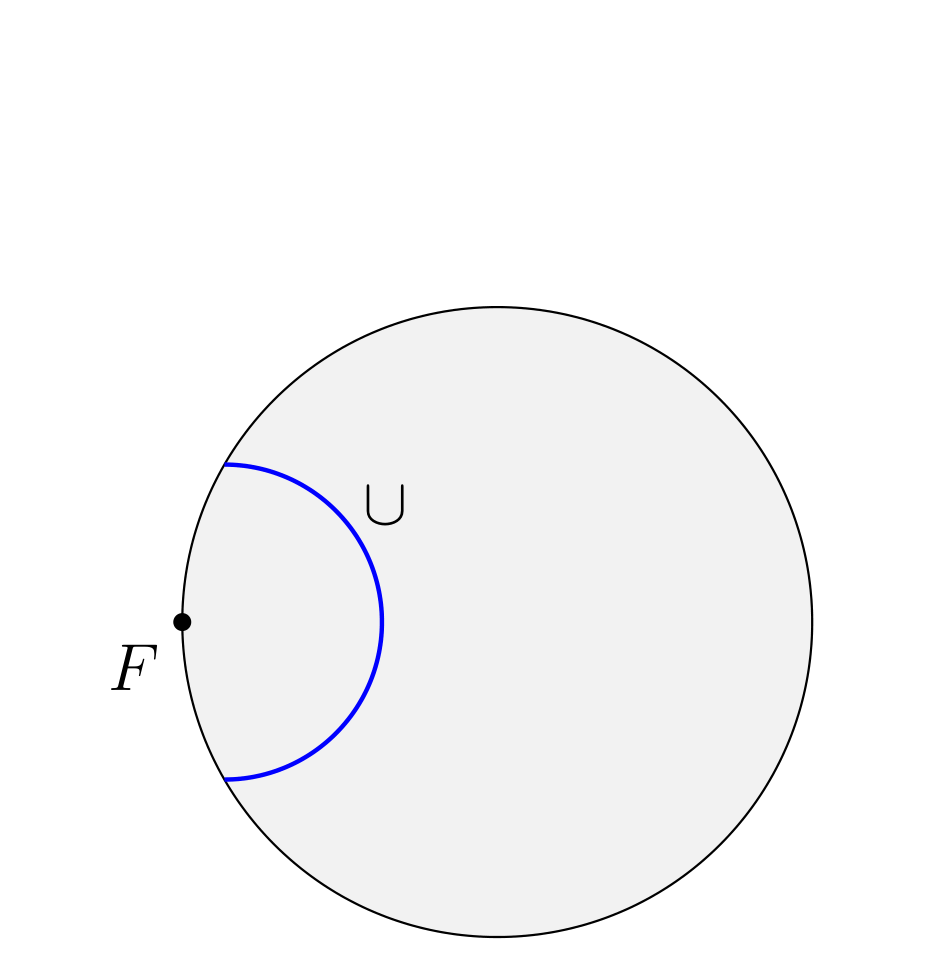
\includegraphics[width=0.40\textwidth]{figures/fig2_1.png}
\caption{cup 函子。}
\label{fig:cup-functor}
\end{figure}

\transnote{背景直觉：cup 函子把停点附近的小拉格朗日盘「绕过一圈」贴到纤维上，形状像把杯子扣在盘子上；cap 是它的形式伴随。}

cup 函子有形式伴随，它由左 Yoneda 模上的拉回 $\operatorname{Mod}\cW(X,F)\to\operatorname{Mod}\cW(F)$ 给出，我们称之为 \textbf{cap 函子}，记作 $\cap$。于是分别有余单位与单位态射 $\eps\colon\cup\cap\to\id$ 与 $\eta\colon\id\to\cap\cup$；把它们补全，就得到双模的正合三角形。这些正合三角形其实可以用 Seidel 早先的工作给出几何刻画：

\begin{thmstar}（Abouzaid--Ganatra, [AG]）\quad 存在双模的正合三角形
\[
\begin{tikzcd}[column sep=2.4em, row sep=1.5em]
\cup\cap \arrow[rr, "\varepsilon"] & & \id \arrow[dl] \\
& \sigma \arrow[ul, "+1"'] &
\end{tikzcd}
\]
（位于 $D^\pi\cW(X,F)$ 上）以及
\[
\begin{tikzcd}[column sep=2.4em, row sep=1.5em]
\cap\cup \arrow[dr, "+1"'] & & \id \arrow[ll, "\eta"] \\
& \mu \arrow[ur, "s"'] &
\end{tikzcd}
\]
（位于 $D^\pi\cW(F)$ 上），其中 $\mu\colon\cW(F)\to\cW(F)$ 是作用在纤维上的顺时针单值性，$\sigma\colon\cW(X,F)\to\cW(X,F)$ 是作用在全空间拉格朗日对象上的顺时针全扭转。此外，自然变换 $s$ 可以等同于 Seidel 的自然变换，后者首见于 [Sei09b]（另见 [Sei08a; Sei17]）。
\end{thmstar}

\transnote{易错预警：本论文第一部分取顺时针约定，与 [GPS20b] 的逆时针缠绕相容；读 [GPS20b] 时容易把 $\mu$ 的方向弄反，可对照 §2.3 的说明。}

本论文定理 \ref{thm:knorrer} 的证明在逻辑上并不需要这条定理；对后文的证明，读者可把 $\mu,\sigma,s$ 取为上文纯代数定义所给出的对象。其中一个三角形的证明梗概见 [AS15, Appendix]。

% ===== 原书 p.44 =====
两个三角形的约定并不相同：本论文第一部分采用的约定与 [GPS20b] 的逆时针缠绕相容，于是存在零次的自然变换 $\id\to\sigma$；这迫使 $\cup,\sigma,\mu$ 都取顺时针方向，且 $\cup$ 为左伴随。然而这样一来，在模型 Lefschetz 纤维丛的情形，$\mu$ 就是负的 Dehn twist 扭转。本论文第二部分则沿用 [Syl19c] 的约定：[Syl19d, Theorem 1.3] 证明，$f$ 绕 $\infty$ 的几何逆时针单值性 $\mu$ 作用在 $\cW(H)$ 上时，等于 $\cup$ 的对偶余扭转再平移 $[2]$；从而 $\mu$ 的镜像将是与线丛 $\cK_X^{-1}|_D$ 作张量。

\transnote{易错预警：在模型 Lefschetz 纤维丛情形，$\mu$ 是负的 Dehn twist 扭转；正负号取决于缠绕方向，不能与第二部分的约定混用。}

现在可以给出定义了：

\begin{defstar}（Auroux，复述第 1 章定义 \ref{def:sing-fuk}）\quad 设奇异辛纤维丛 $f\colon X\to\C$ 恰有一个奇异纤维，位于 $0$ 上方。则 $f^{-1}(0)$ 的 wrapped Fukaya 范畴定义为：在自然变换 $s\colon\mu\to\id$ 处，取 $t\neq0$ 充分小时的邻近纤维 $f^{-1}(t)$ 的 wrapped Fukaya 范畴的局部化：
\[
D\cW(f^{-1}(0))=D\cW(f^{-1}(t))[s^{-1}].
\]
\end{defstar}

\transnote{含糊点拨：原书把第 1 章的那条定义（定义 \ref{def:sing-fuk}）原样复述，编号也保持不变。此处的译文按引用式复述处理，不占本章编号。}

条件“$|t|\neq0$ 充分小”是为了排除 $t$ 是 Malgrange 条件失效点的可能；§2 前面的定义已把这类点排除在 Landau--Ginzburg 模型之外。

% ===== 原书 p.45 =====
注意，这一定义等价于对范畴 $\cW(f^{-1}(t))$ 取商，商掉由该自然变换的各锥构成的满子范畴；也就是说，商掉复合 $\cap\cup$ 的本质像。下面这条引理在计算中常常有用：

\begin{lemma}\label{lem:essential-image}\label{lem:2-3-1}
复合 $\cap\cup$ 的本质像与 $\cap$ 的本质像有相同的分裂闭包。
\end{lemma}

\begin{proof}
一个包含关系是显然的。为证反向包含，考虑联系 $\cap$ 与 $\cup$ 之复合的两个正合三角形；须注意，按上面的约定，这两个三角形的箭头方向相反，其中 $\eps$ 与 $\eta$ 分别是 $\cup$--$\cap$ 伴随的余单位与单位。我们对第一个三角形作用 $\cap$，并在第二个三角形前复合 $\cap$。由正合性以及恒等式 $\mu\cap=\cap\sigma$ [AG]，得到两个三角形：
\[
\begin{tikzcd}[column sep=3.2em, row sep=1.5em]
\cap\cup\cap \arrow[rr, "\cap\varepsilon"] & & \cap \arrow[dl] \\
& \mu\cap \arrow[ul, "+1"'] &
\end{tikzcd}
\]
\[
\begin{tikzcd}[column sep=3.2em, row sep=1.5em]
\cap\cup\cap \arrow[dr, "+1"'] & & \cap \arrow[ll, "\eta\cap"] \\
& \mu\cap \arrow[ur] &
\end{tikzcd}
\]
伴随的单位–余单位恒等式 $\cap\eps\circ\eta\cap=\id_{\cap}$ 说明第二个三角形中的映射 $\mu\cap\to\cap$ 为零，故该三角形分裂。于是 $\cap\cup\cap L$ 总以 $\cap L$ 为直和项。
\end{proof}

\transnote{易错预警：两个三角形的箭头方向相反；须先对第一个作用 $\cap$，再给第二个前复合 $\cap$，顺序颠倒会得到不同的三角形。}

% ===== 原书 p.46 =====
\begin{figure}[htbp]
\centering
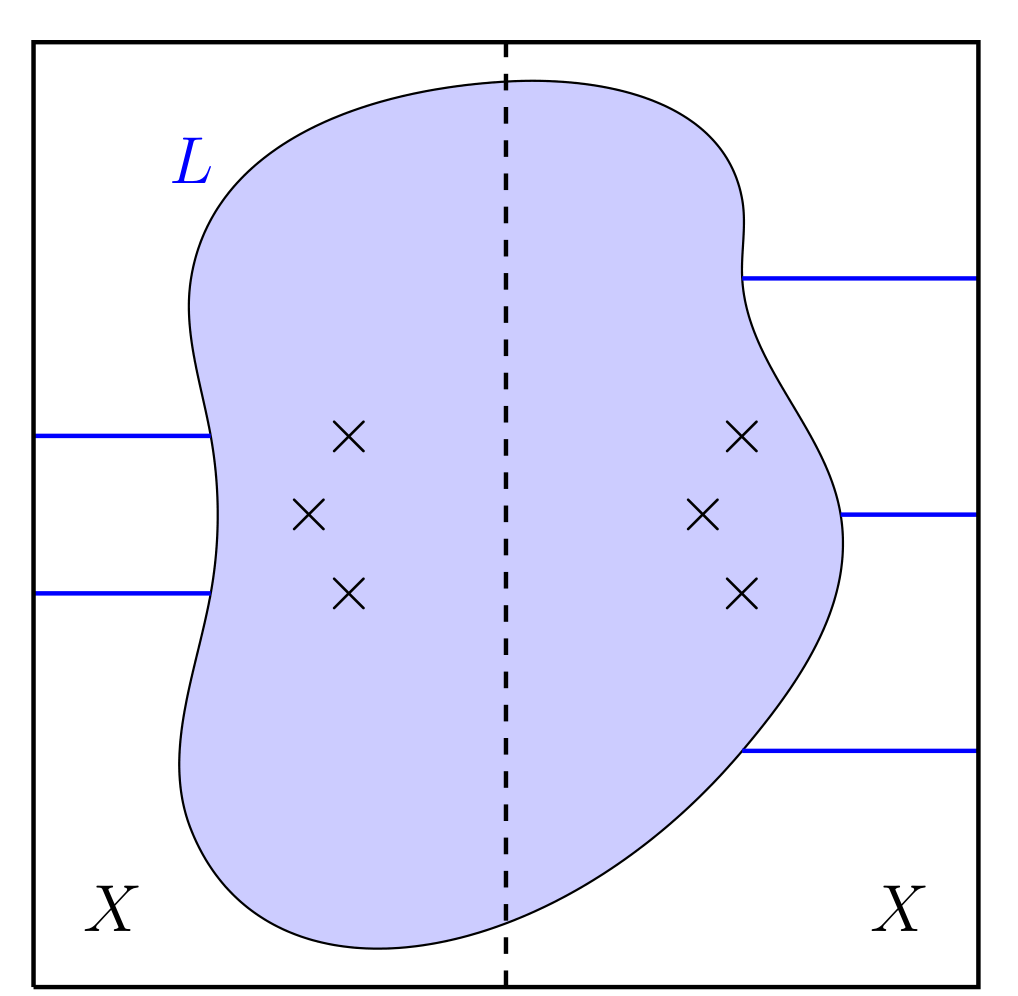
\includegraphics[width=0.52\textwidth]{figures/fig2_2.png}
\caption{拼接起来的若干份 $X$ 内部的拉格朗日配边 $L$。}
\label{fig:cobordism}
\end{figure}

\begin{remarkx}\label{rem:7}
要看出定理 \ref{thm:knorrer} 中取扭复形的分裂闭包是必要的，可考虑如下情形：绕奇异纤维的单值性由绕同一 vanishing cycle 的两个 Dehn twist 扭转之复合给出。
\end{remarkx}

\transnote{背景直觉：取分裂闭包是为让锥在幂等分裂下封闭；绕同一消失圈复合两次 Dehn twist 扭转时，缺了它范畴就会漏掉直和项。}

\begin{corollary}\label{cor:sing-fuk-quotient}\label{cor:2-3-2}
范畴 $D^\pi\cW(f^{-1}(0))$ 拟等价于 $D^\pi\cW(f^{-1}(t))$ 商掉 $\cap$ 的本质像所得的商范畴。
\end{corollary}

\begin{proof}
由引理 \ref{lem:essential-image}，函子 $\cap\cup$ 与 $\cap$ 的本质像有相同的分裂闭包，因此所得的两个商范畴彼此拟等价。
\end{proof}

若读者希望避开 [AG]，也可在证明定理 \ref{thm:knorrer} 时改把推论 \ref{cor:sing-fuk-quotient} 当作定义。

定义 \ref{def:sing-fuk} 与辛纤维丛内部的拉格朗日配边还有一层特别自然的关系（参看 [BC17]）。代替研究乘积 $f^{-1}(t)\times\C$ 中的拉格朗日配边，我们可以改为考虑 $X$ 内部（或若干个 $X$ 拼接起来）的拉格朗日配边，只要求其两端经 $f$ 投影到与正实轴或负实轴平行的射线上：见图 \ref{fig:cobordism}。在作一次哈密顿同痕之后，每条这样的配边都可以只看作只有正端；于是这些零配边给出了拉格朗日配边群上全部的关系。而这些关系说的正是：$\cap$ 的像中的每个复形都必须等价于零。由推论 \ref{cor:sing-fuk-quotient}，这正是深谷范畴 $\cW(f^{-1}(0))$ 的等价描述。因此我们猜想，这一构造刻画了 Grothendieck 群 $K_0(D^\pi\cW(f^{-1}(0)))$。

\transnote{含糊点拨：原文此处是 conjecture，作者并未证明，引用时不可当作定理；它把配边群与 $K_0$ 联系起来。}
% ===== 原书 p.47 =====
